% Options for packages loaded elsewhere
\PassOptionsToPackage{unicode}{hyperref}
\PassOptionsToPackage{hyphens}{url}
\PassOptionsToPackage{dvipsnames,svgnames,x11names}{xcolor}
\documentclass[
  10pt,
  a4paper]{article}
\usepackage{xcolor}
\usepackage[margin=1in]{geometry}
\usepackage{amsmath,amssymb}
\setcounter{secnumdepth}{5}
\usepackage{iftex}
\ifPDFTeX
  \usepackage[T1]{fontenc}
  \usepackage[utf8]{inputenc}
  \usepackage{textcomp} % provide euro and other symbols
\else % if luatex or xetex
  \usepackage{unicode-math} % this also loads fontspec
  \defaultfontfeatures{Scale=MatchLowercase}
  \defaultfontfeatures[\rmfamily]{Ligatures=TeX,Scale=1}
\fi
\usepackage{lmodern}
\ifPDFTeX\else
  % xetex/luatex font selection
\fi
% Use upquote if available, for straight quotes in verbatim environments
\IfFileExists{upquote.sty}{\usepackage{upquote}}{}
\IfFileExists{microtype.sty}{% use microtype if available
  \usepackage[]{microtype}
  \UseMicrotypeSet[protrusion]{basicmath} % disable protrusion for tt fonts
}{}
\makeatletter
\@ifundefined{KOMAClassName}{% if non-KOMA class
  \IfFileExists{parskip.sty}{%
    \usepackage{parskip}
  }{% else
    \setlength{\parindent}{0pt}
    \setlength{\parskip}{6pt plus 2pt minus 1pt}}
}{% if KOMA class
  \KOMAoptions{parskip=half}}
\makeatother
\usepackage{longtable,booktabs,array}
\newcounter{none} % for unnumbered tables
\usepackage{calc} % for calculating minipage widths
% Correct order of tables after \paragraph or \subparagraph
\usepackage{etoolbox}
\makeatletter
\patchcmd\longtable{\par}{\if@noskipsec\mbox{}\fi\par}{}{}
\makeatother
% Allow footnotes in longtable head/foot
\IfFileExists{footnotehyper.sty}{\usepackage{footnotehyper}}{\usepackage{footnote}}
\makesavenoteenv{longtable}
\usepackage{graphicx}
\makeatletter
\newsavebox\pandoc@box
\newcommand*\pandocbounded[1]{% scales image to fit in text height/width
  \sbox\pandoc@box{#1}%
  \Gscale@div\@tempa{\textheight}{\dimexpr\ht\pandoc@box+\dp\pandoc@box\relax}%
  \Gscale@div\@tempb{\linewidth}{\wd\pandoc@box}%
  \ifdim\@tempb\p@<\@tempa\p@\let\@tempa\@tempb\fi% select the smaller of both
  \ifdim\@tempa\p@<\p@\scalebox{\@tempa}{\usebox\pandoc@box}%
  \else\usebox{\pandoc@box}%
  \fi%
}
% Set default figure placement to htbp
\def\fps@figure{htbp}
\makeatother
\setlength{\emergencystretch}{3em} % prevent overfull lines
\providecommand{\tightlist}{%
  \setlength{\itemsep}{0pt}\setlength{\parskip}{0pt}}
\usepackage[utf8]{inputenc}
\usepackage[spanish, es-tabla, es-nodecimaldot]{babel}
\usepackage{actuarialsymbol}
\usepackage{multicol}
\usepackage{multirow}
\usepackage{setspace}
\usepackage{graphicx}
\usepackage{float}
\usepackage{subfigure}
\usepackage{url}
\usepackage{enumitem}
\usepackage{mathrsfs}
\usepackage{amsmath}
\usepackage{amsfonts}
\usepackage{amssymb}
\usepackage{makeidx}
\usepackage{listings}
\usepackage{flushend}
\usepackage{caption}
\usepackage{minted}
\usepackage{booktabs}
\usepackage[none]{hyphenat}
\usepackage{latexsym}
\usepackage{dsfont}
\newcommand{\R}{\mathbb{R}}
\newcommand{\N}{\mathbb{N}}
\usepackage{ragged2e}
\usepackage{array}
\renewcommand{\contentsname}{Índice}
\usepackage{schemata}
\usepackage{graphicx}
\newcommand\diagram[2]{\schema{\schemabox{#1}}{\schemabox{#2}}}
\usepackage{hyperref}
\usepackage{color}
\definecolor{gris}{RGB}{70,70,70}
\definecolor{negro}{RGB}{40,40,40}
\definecolor{brinkpink}{rgb}{0.98, 0.38, 0.5}
\definecolor{richlavender}{rgb}{0.67, 0.38, 0.8}
\newcommand{\colorhrule}[3]{\begingroup\color{#1}\rule{#2}{#3}\endgroup}
\setlength{\intextsep}{1mm}
\setlength{\columnsep}{5mm}
\usepackage{hyperref}
\usepackage{booktabs}
\usepackage{longtable}
\usepackage{array}
\usepackage{multirow}
\usepackage{wrapfig}
\usepackage{float}
\usepackage{colortbl}
\usepackage{pdflscape}
\usepackage{tabu}
\usepackage{threeparttable}
\usepackage{threeparttablex}
\usepackage[normalem]{ulem}
\usepackage{makecell}
\usepackage{xcolor}
\usepackage{bookmark}
\IfFileExists{xurl.sty}{\usepackage{xurl}}{} % add URL line breaks if available
\urlstyle{same}
\hypersetup{
  colorlinks=true,
  linkcolor={blue},
  filecolor={Maroon},
  citecolor={Blue},
  urlcolor={blue},
  pdfcreator={LaTeX via pandoc}}

\author{}
\date{\vspace{-2.5em}}

\begin{document}

\sloppy
\begin{center}
\begin{tabular}{cc}
\multirow{2}{3.5cm}{
\includegraphics[width=2.5cm]{logofc.png}}  & \large{\textsc{Universidad Nacional Autónoma de México}}\\\vspace{5mm}
 & \normalsize{Facultad de Ciencias}\\\vspace{5mm}
 
 & \normalsize{\textbf{Diplomado Introducción Analítica a la Ciencia de Datos}}\\ 
 \vspace{.3cm}
 & \vspace{.3cm}\normalsize{Módulo VI: Aprendizaje no supervisado}\\ \vspace{0.1cm}
 & \small{Profesor: Salvador Zamora Muñoz} 
 %\\ %\vspace{.1cm}
 %& \small{ Jorge Ignacio González Cázares}
\end{tabular}
\end{center}

\vspace{.1cm}

\begin{center}
\begingroup\color{negro}\rule{16cm}{1.2pt}\endgroup

\vspace{.4cm}

\textbf{Proyecto 1}

\vspace{0.2cm}

Técnicas de reducción de dimensión: PC, t-SNE y UMAP.

%\textbf{Proyecto 2}

%\vspace{0.2cm}

%Técnicas de agrupamiento o clustering: Clusters por métodos aglomerativos y por método de K-MEANS.

\vspace{.4cm}

\begingroup\color{negro}\rule{16cm}{1.2pt}\endgroup
\end{center}

\vspace{0.2cm}

\begin{center}
\textbf{Equipo 6}
\end{center}

\vspace{0.2cm}

\begin{table}[h]
    \centering
    \renewcommand{\arraystretch}{1.5} % Aumenta el espacio entre filas
    \begin{tabular}{lc}
        \textbf{Integrantes} & \textbf{Opción de titulación}\\
        Betancourt Peralta Diego & Sí\\
        Canul Hernández Erick Iván & Sí\\
        Gutiérrez Gutiérrez José Omar & Sí\\
        Hernández Pérez Maximiliano & \\
        Torres Vargas Brenda Poulette & Sí \\
    \end{tabular}
\end{table}

\thispagestyle{empty}

\clearpage

\tableofcontents

\clearpage

\title{Reducción de Dimensionalidad}

\section{Planteamiento del Problema}\label{planteamiento-del-problema}

Si bien durante los procesos de admisión a posgrado diversos factores académicos y personales, como el desempeño en exámenes, el promedio general de la licenciatura, la calidad de la institución de procedencia, las cartas de recomendación, la declaración de propósitos y la experiencia en investigación, impactan en la probabilidad de que un aspirante sea admitido, dichos factores pueden presentar distintos niveles de correlación y redundancia, de modo que resulta pertinente analizar su estructura mediante técnicas de reducción de dimensión para identificar las variables que aportan mayor información, simplificar el espacio de características y facilitar la interpretación de los datos sin perder una cantidad significativa de información.

En este sentido, analizamos el conjunto de datos de \textbf{Admission Predict}, integrado por 400 observaciones correspondientes a solicitudes de admisión y 8 variables, de las cuales 7 corresponden a variables predictoras y una a la variable respuesta. A continuación, se presenta una breve descripción de las mismas:

\begin{itemize}
\tightlist
\item
  \textbf{\texttt{GRE\ Score}}: puntuación obtenida en el examen GRE (0--340).
\item
  \textbf{\texttt{TOEFL\ Score}}: puntuación obtenida en el examen TOEFL (0--120).
\item
  \textbf{\texttt{University\ Rating}}: calificación de la universidad de procedencia (escala de 1 a 5).
\item
  \textbf{\texttt{SOP}}: evaluación de la declaración de propósito (Statement of Purpose), en una escala de 1 a 5.
\item
  \textbf{\texttt{LOR}}: evaluación de las cartas de recomendación (Letter of Recommendation), en una escala de 1 a 5.
\item
  \textbf{\texttt{CGPA}}: promedio general de licenciatura, expresado en una escala de 0 a 10.
\item
  \textbf{\texttt{Research}}: variable binaria que representa si el aspirante cuenta (1) o no (0) con experiencia en investigación.
\item
  \textbf{\texttt{Chance\ of\ Admit}}: Variable continua acotada en el intervalo \(\lbrack 0,1\rbrack\), que representa la probabilidad estimada de
\end{itemize}

\section{Estadística Descriptiva}\label{estaduxedstica-descriptiva}

En la figura \ref{fig:scattercontinuas} observamos una relación positiva entre la variable Chance of Admit y el resto de variables continuas (GRE Score, TOEFL Score y CGPA), por lo que los alumnos con mejores calificaciones en el examen GRE, TOEFL y mejor GPA tienen más probabilidad de ser admitidos en el programa de maestría de su elección.

\begin{figure}[ht]

{\centering 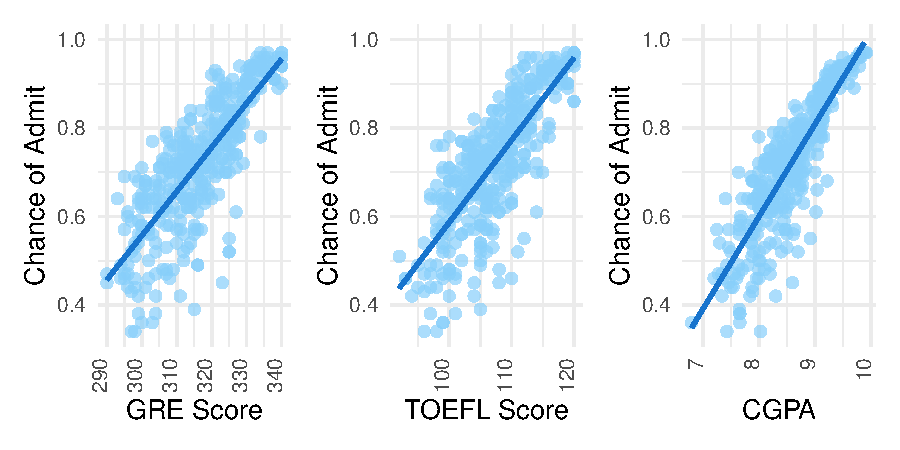
\includegraphics{proyecto-reduccion-dimensionalidad_files/figure-latex/scattercontinuas-1} 

}

\caption{Relación entre las variables continuas y Chance of Admit}\label{fig:scattercontinuas}
\end{figure}

En la figura \ref{fig:boxplotscategoricas} se tiene un boxplot de Chance of Admit por cada categoría de cada una de las variables categóricas (University Rating, SOP, LOR y Research).

\begin{figure}[ht]

{\centering 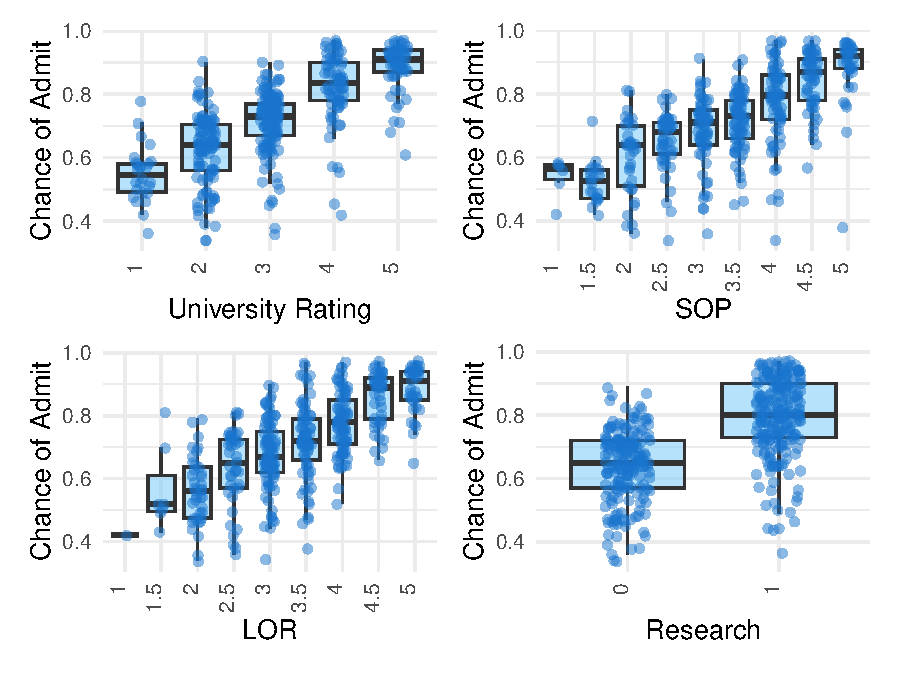
\includegraphics{proyecto-reduccion-dimensionalidad_files/figure-latex/boxplotscategoricas-1} 

}

\caption{Boxplots de Chance of Admit por cada categoría de las variables categóricas}\label{fig:boxplotscategoricas}
\end{figure}

En la figura \ref{fig:matrizcorr} observamos en la matriz de correlación de Pearson que todas las variables están correlacionadas entre sí de manera positiva. Todas las correlaciones son de al menos 0.4, por lo que hay una estructura de asociación lineal fuerte entre las variables.

\begin{figure}[ht]

{\centering 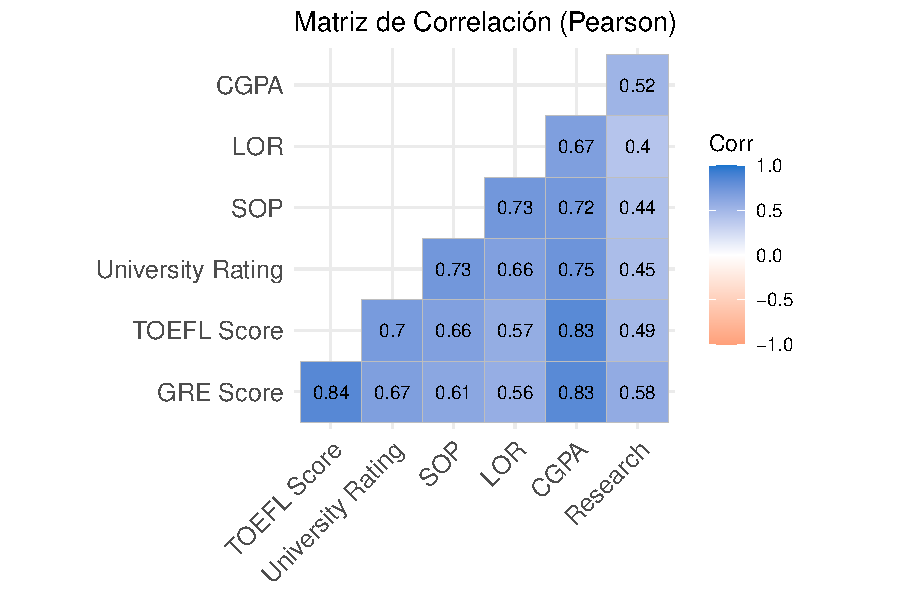
\includegraphics{proyecto-reduccion-dimensionalidad_files/figure-latex/matrizcorr-1} 

}

\caption{Matriz de correlación}\label{fig:matrizcorr}
\end{figure}

Así mismo, la matriz de correlación tiene un determinante de 0.0033, lo cual confirma todavía más la fuerte correlación entre las variables.

La medida de adecuación muestral (MSA por sus siglas en inglés) de Kaiser, Meyer, Olkin (KMO) es un valor que va de 0 a 1 y que es útil para medir qué tan adecuado es realizar un análisis de componentes principales con los datos de interés. Valores mayores indican que es conveniente realizar un análisis de este tipo con los datos. El valor obtenido con estos datos fue de 0.903, por lo que realizar un análisis de componentes principales es apropiado.

\section{Aplicación de las Técnicas de Reducción de Dimensión}\label{aplicaciuxf3n-de-las-tuxe9cnicas-de-reducciuxf3n-de-dimensiuxf3n}

\subsection{PCA}\label{pca}

El análisis de componentes principales se aplicó sobre el conjunto de variables predictoras estandarizadas mediante el procedimiento de normalización, integrando tanto las variables cuantitativas: \texttt{GRE Score}, \texttt{TOEFL Score}, \texttt{University Rating}, \texttt{SOP}, \texttt{LOR} y \texttt{CGPA}, como la variable categórica \texttt{Research}, la cual fue convertida a tipo factor con dos niveles (No y Sí). No obstante, \texttt{Chance of Admit} se excluyó del cálculo, asignándole el rol de \textit{outcome} y se conservó únicamente para facilitar la interpretación posterior de los resultados.

Así pues, una vez extraídos los componentes principales, se obtuvo su matriz de cargas factoriales, que se muestra en la tabla \ref{tab:varianzapca}, las cuales indican la contribución de cada variable original a la construcción de cada componente, así como su matriz de varianza explicada asociada a cada uno y la acumulada en términos porcentuales, la cual se muestra en la tabla \ref{tab:porcentajevar}.

\vspace{.4cm}

\begin{table}[!h]
\centering
\caption{\label{tab:varianzapca}Matriz de cargas factoriales absolutas de los componentes principales}
\centering
\resizebox{\ifdim\width>\linewidth\linewidth\else\width\fi}{!}{
\begin{tabular}[t]{cccccccc}
\toprule
\textbf{Variable} & \textbf{PC1} & \textbf{PC2} & \textbf{PC3} & \textbf{PC4} & \textbf{PC5} & \textbf{PC6} & \textbf{PC7}\\
\midrule
CGPA & \cellcolor[HTML]{A1D769}{\textcolor{black}{0.4174}} & \cellcolor[HTML]{FFFCBA}{\textcolor{black}{-0.0206}} & \cellcolor[HTML]{FED581}{\textcolor{black}{-0.2452}} & \cellcolor[HTML]{E4F49A}{\textcolor{black}{0.1407}} & \cellcolor[HTML]{FFF9B6}{\textcolor{black}{-0.0358}} & \cellcolor[HTML]{F57145}{\textcolor{black}{-0.5876}} & \cellcolor[HTML]{5CB760}{\textcolor{black}{0.6316}}\\
GRE Score & \cellcolor[HTML]{A6D96A}{\textcolor{black}{0.3982}} & \cellcolor[HTML]{FECA78}{\textcolor{black}{-0.2874}} & \cellcolor[HTML]{FEB96A}{\textcolor{black}{-0.3553}} & \cellcolor[HTML]{D8EF8A}{\textcolor{black}{0.2039}} & \cellcolor[HTML]{FFF6B0}{\textcolor{black}{-0.0592}} & \cellcolor[HTML]{FECD7B}{\textcolor{black}{-0.2752}} & \cellcolor[HTML]{E44D33}{\textcolor{black}{-0.7154}}\\
LOR & \cellcolor[HTML]{B1DE71}{\textcolor{black}{0.356}} & \cellcolor[HTML]{97D268}{\textcolor{black}{0.4495}} & \cellcolor[HTML]{A2D76A}{\textcolor{black}{0.4134}} & \cellcolor[HTML]{69BE63}{\textcolor{black}{0.5922}} & \cellcolor[HTML]{FEBC6D}{\textcolor{black}{-0.344}} & \cellcolor[HTML]{DFF293}{\textcolor{black}{0.1681}} & \cellcolor[HTML]{FFF6B1}{\textcolor{black}{-0.0552}}\\
Research Yes & \cellcolor[HTML]{C2E57C}{\textcolor{black}{0.2915}} & \cellcolor[HTML]{E24A31}{\textcolor{black}{-0.7239}} & \cellcolor[HTML]{63BB62}{\textcolor{black}{0.6084}} & \cellcolor[HTML]{FFF5AE}{\textcolor{black}{-0.0666}} & \cellcolor[HTML]{FFFEBD}{\textcolor{black}{-0.0079}} & \cellcolor[HTML]{F1F9AC}{\textcolor{black}{0.0747}} & \cellcolor[HTML]{EBF7A4}{\textcolor{black}{0.1038}}\\
SOP & \cellcolor[HTML]{ABDB6D}{\textcolor{black}{0.3822}} & \cellcolor[HTML]{B3DE72}{\textcolor{black}{0.3505}} & \cellcolor[HTML]{CBE982}{\textcolor{black}{0.2569}} & \cellcolor[HTML]{FEDC88}{\textcolor{black}{-0.2143}} & \cellcolor[HTML]{2C9E53}{\textcolor{black}{0.7676}} & \cellcolor[HTML]{FFF0A5}{\textcolor{black}{-0.0989}} & \cellcolor[HTML]{FFE99A}{\textcolor{black}{-0.1421}}\\
TOEFL Score & \cellcolor[HTML]{A6D96A}{\textcolor{black}{0.3989}} & \cellcolor[HTML]{FFEC9F}{\textcolor{black}{-0.1231}} & \cellcolor[HTML]{FB9D59}{\textcolor{black}{-0.4545}} & \cellcolor[HTML]{EFF8AA}{\textcolor{black}{0.0828}} & \cellcolor[HTML]{DFF293}{\textcolor{black}{0.1687}} & \cellcolor[HTML]{3BA557}{\textcolor{black}{0.7299}} & \cellcolor[HTML]{D2EC87}{\textcolor{black}{0.2261}}\\
University Rating & \cellcolor[HTML]{A9DA6C}{\textcolor{black}{0.3877}} & \cellcolor[HTML]{D1EC86}{\textcolor{black}{0.2301}} & \cellcolor[HTML]{FEFEBD}{\textcolor{black}{0.0064}} & \cellcolor[HTML]{E24931}{\textcolor{black}{-0.7285}} & \cellcolor[HTML]{F98C50}{\textcolor{black}{-0.509}} & \cellcolor[HTML]{F5FBB2}{\textcolor{black}{0.0513}} & \cellcolor[HTML]{FFF5AE}{\textcolor{black}{-0.065}}\\
\bottomrule
\end{tabular}}
\end{table}

\vspace{.4cm}

\begin{table}[!h]
\centering
\caption{\label{tab:porcentajevar}Matriz de cargas factoriales absolutas de los componentes principales}
\centering
\resizebox{\ifdim\width>\linewidth\linewidth\else\width\fi}{!}{
\begin{tabular}[t]{ccc}
\toprule
PC & Varianza explicada (\%) & Acumulada (\%)\\
\midrule
1 & 69.61 & 69.61\\
2 & 10.36 & 79.97\\
3 & 7.81 & 87.78\\
4 & 4.43 & 92.21\\
5 & 3.50 & 95.71\\
6 & 2.27 & 97.98\\
7 & 2.02 & 100.00\\
\bottomrule
\end{tabular}}
\end{table}

Notemos que el primer componente principal \textbf{(PC1) concentra 69.61\%} de la variabilidad total del conjunto de datos, lo que indica que una gran parte de la información contenida en las siete variables predictoras puede resumirse en una única dimensión latente. Por otra parte, al incorporar el segundo componente principal \textbf{(PC2), la varianza acumulada asciende a 79.97\%}, lo que representa aproximadamente el 80\% de la variabilidad total. Asimismo, con la inclusión del tercer componente principal \textbf{(PC3) se alcanza una varianza acumulada de 87.78\%}, mientras que los componentes restantes aportan incrementos relativamente pequeños, inferiores al 5\% de manera individual.

De modo que los resultados muestran que la mayor parte de la información del conjunto de datos se encuentra concentrada en los primeros componentes principales, lo que confirma la existencia de correlación entre las variables originales. Ahora bien, considerando el criterio de conservar alrededor del 80\% de la varianza explicada, se concluye que \textbf{dos componentes principales son suficientes para representar adecuadamente la estructura de los datos}, permitiendo reducir el número de dimensiones de siete a dos con una pérdida mínima de información.

En cuanto a las cargas factoriales, observamos que el PC1 presenta cargas de magnitud similar para todas las variables predictoras, siendo ligeramente mayor para \texttt{CGPA} (0.417), seguida de \texttt{TOEFL Score} (0.399), \texttt{GRE Score} (0.398) y \texttt{University Rating} (0.388), lo que sugiere que el primer componente resume un factor asociado al desempeño académico general de los postulantes, mientras que en el PC2 domina la variable \texttt{Research} con una carga absoluta de 0.724, superando ampliamente a la del resto de las variables, indicando que el segundo componente captura principalmente la variabilidad asociada a la experiencia en investigación, mientras que variables como \texttt{LOR} (0.449), \texttt{GRE Score} (0.287) y \texttt{University Rating} (0.230) presentan una contribución moderada.

Ahora bien, al proyectar a los postulantes sobre el plano definido por PC1 y PC2 (figura \ref{fig:pcagrafica}), coloreando cada punto según su \texttt{Chance of Admit}, se observa un gradiente claro a lo largo del eje PC1: los estudiantes con mayor probabilidad de admisión se concentran en la región de valores negativos de PC1, mientras que aquellos con menor probabilidad se agrupan principalmente en la región de valores positivos.

\begin{figure}[ht]

{\centering 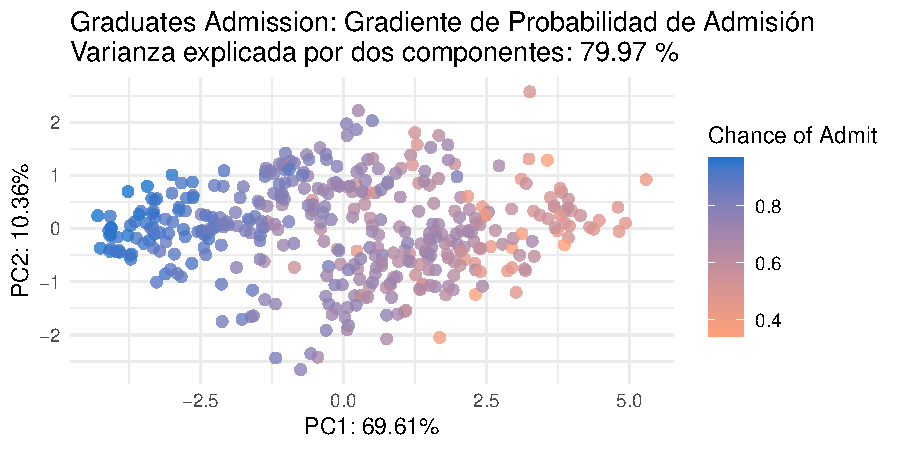
\includegraphics{proyecto-reduccion-dimensionalidad_files/figure-latex/pcagrafica-1} 

}

\caption{Proyección de los postulantes sobre PC1 y PC2, coloreada según la probabilidad de admisión}\label{fig:pcagrafica}
\end{figure}

Este patrón resulta consistente con la interpretación anterior de PC1 como un factor asociado al desempeño académico general, y resulta particularmente relevante dado que \texttt{Chance of Admit} no participó en el cálculo de los componentes, lo cual sugiere que la estructura de correlación capturada de forma no supervisada por el PCA coincide, en buena medida, con el resultado que en la práctica resulta más relevante para el proceso de admisión.

De manera complementaria, al segmentar a los postulantes según su experiencia en investigación (figura \ref{fig:researchpca}) se observa una separación clara a lo largo del eje PC2: los estudiantes con experiencia en investigación (\texttt{Sí}) se concentran principalmente en la región de valores positivos de PC2, mientras que aquellos sin experiencia (\texttt{No}) se ubican mayoritariamente en la región de valores negativos, sin que se aprecie una separación equivalente a lo largo de PC1.

\begin{figure}[ht]

{\centering 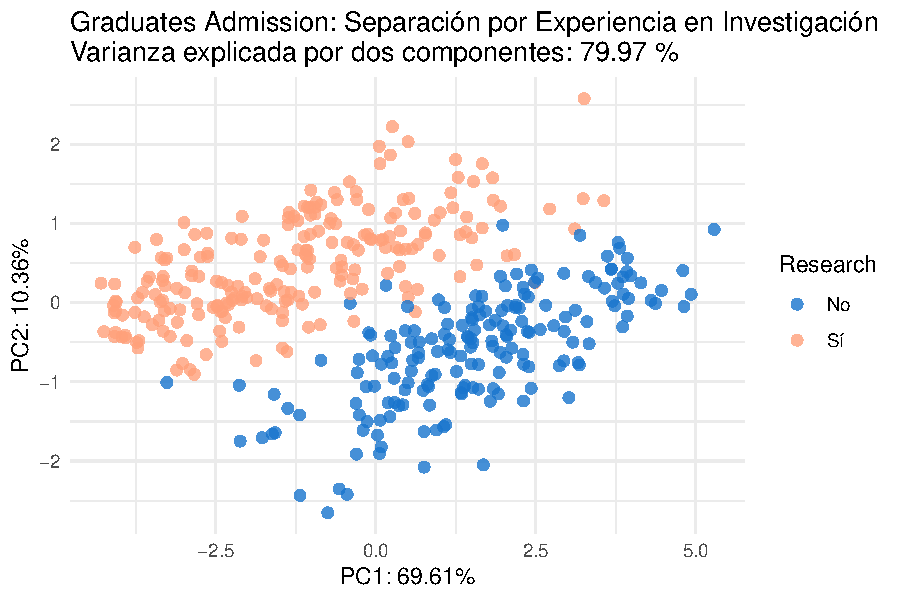
\includegraphics{proyecto-reduccion-dimensionalidad_files/figure-latex/researchpca-1} 

}

\caption{Proyección de los postulantes sobre PC1 y PC2, segmentada según experiencia en investigación}\label{fig:researchpca}
\end{figure}

Así pues, es posible concluir que la variabilidad original contenida en las siete variables predictoras puede resumirse de manera adecuada en dos dimensiones interpretables: \textbf{una asociada al desempeño académico} y \textbf{otra a la experiencia en investigación}, las cuales en conjunto \textbf{retienen el 79.97\% de la información total}.

\end{document}
